% Created 2026-05-14 Thu 18:05
% Intended LaTeX compiler: pdflatex
\documentclass[11pt]{article}

\usepackage[utf8]{inputenc}
\usepackage[T1]{fontenc}
\usepackage{graphicx}
\usepackage{longtable}
\usepackage{wrapfig}
\usepackage{rotating}
\usepackage[normalem]{ulem}
\usepackage{amsmath}
\usepackage{amssymb}
\usepackage{capt-of}
\usepackage{hyperref}
\usepackage{minted}
\usepackage{tabularx}
\usepackage{tabularx}
\author{flavio}
\date{\today}
\title{Interfacce}
\hypersetup{
 pdfauthor={flavio},
 pdftitle={Interfacce},
 pdfkeywords={},
 pdfsubject={},
 pdfcreator={},
 pdflang={English}}
\begin{document}

\maketitle
\tableofcontents

\section{Cos'è una interfaccia}
\label{sec:orgbd290fd}
Le interfacce vengono usate per consentire a più classi di fornire e implementare più metodi comuni. Le interfacce definiscono e standardizzano l'interazione fra oggetti tramite un insieme di metodi comuni. Le interfacce sono classi astratte.
\section{Dichiarazione di una interfaccia}
\label{sec:orgbde68e4}
Le interfacce sono classi astratte. Tutti i metodi delle interfacce sono astratti e non si possono definire implementazioni, anche se da Java 9 è possibile definire delle implementazioni di default dei metodi con la parola chiave \texttt{default}. I campi sono costanti \texttt{final public static}. Si possono dichiarare metodi private per il riuso del codice.

\begin{minted}[]{java}
public interface SupportoRiscrivibile{
    int TIMES = 100;
    void leggi();
    void scrivi();
}
\end{minted}

\begin{minted}[]{java}

public class Nastro implements SupportoRiscrivibile{
    private Pellicola pellicola;
    @Override
    public void leggi(){
        attivaTestina();
        muoviTestina();
    }
    @Override
    public void scrivi(){
        attivaTestina();
        caricaTestina();
        muoviTestina();
        scaricaTestina();
    }
    public void attivaTestina(){}
    public void caricaTestina(){}
    public void scaricaTestina(){}
    public void muoviTestina(){}
}

\end{minted}
\subsection{metodi di default}
\label{sec:orge212901}

\begin{minted}[]{java}

public interface Loggabile{
    // loglevel è una enum probabilmente
    private void log(String msg, LogLevel level)
        {
            ...
        }
    default void logInfo(String msg) {log(msg,LogLevel.INFO)}
    default void logWarn(String msg) {log(msg,LogLevel.WARNING)}
    default void logError(String msg) {log(msg, LogLeve.ERROR)}
}

\end{minted}
\section{Perché usare una interfaccia?}
\label{sec:org4c721f5}
Le interfacce permettono di modellare comportamenti comuni a classi che non sono in relazione gerarchica. Inoltre una classe può ereditare da più interfacce, le
\subsection{Problema del diamante}
\label{sec:orgf9caa31}
Java non possiede meccanismi per l'ereditarietà multipla,per buone ragioni: si possono creare situazioni poco chiare di duplicazione di metodi e campi. Uno dei problemi che sorge in pratica è il problema del diamante.

Ad esempio:
\begin{center}
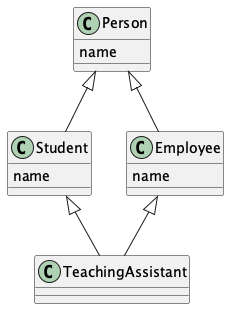
\includegraphics[width=.9\linewidth]{diamante.png}
\label{}
\end{center}

Qui TeachingAssistant eredita da Student ed Employee due campi con lo stesso nome e questa genera ambiguità. In java l'eredità multipla non esiste con le classi ma si può ripresentare con le interfacce. Se le interfacce hanno 2 metodi di default allora bisogna scegliere quello che vogliamo chiamare o reimplemntarlo noi:

\begin{minted}[]{java}
public interface A{
    void ciao() {System.out.println("ciao da A");}
}
public interface B{
    void ciao(){System.out.println("ciao da B");}
}

public class C implments A,B {
    @Override
    void ciao(){
        A.super.ciao();
    }
}
\end{minted}
\section{Interfacce notevole}
\label{sec:org5cc571d}
\begin{center}
\begin{tabularx}{\textwidth}{lX}
Interfaccia & Descrizione\\
\hline
Comparable & Impone un ordinamento naturale degli oggetti tramite il metodo: int compareTo(T b), che restituisce un valore >, =,  < 0 se l'oggetto è rispettivamente maggiore, uguale o minore di b\\
Clonable & Le classi che implementano quest'interfaccia dichiarano al metodo clone() che si può fare una copia campo-campo delle istanze.\\
Serializable & Questa interfaccia non possiede metodi o campi e serve soltanto ad identificare il fatto che l'oggetto è serializzabile, ciòe: memorizzabile su un supporto\\
\hline
\end{tabularx}
\end{center}
\section{Le interfacce Iterable e java.util.Iterator}
\label{sec:orgcca4b6f}
Le interafface Iterable e Iterator permettono di avere iterare sugli oggetti di tipo collection.
\subsection{Iterable}
\label{sec:org3a38bf7}
Un'interfaccia fondamentale che permette di iterare su collezioni.
ha come metodi:
\begin{center}
\begin{tabular}{ll}
Metodo & Descrizione\\
\hline
boolean hasNext() & Restituisce true se esiste ancora un elemento nella collezione\\
E next() & Restituisce l'elemento successivo\\
void remove() & rimuove l'elemento corronte\\
\hline
\end{tabular}
\end{center}


\begin{minted}[]{java}

import java.util.ArrayList;
import java.util.Iterator;

public class Jukebox{
    private ArrayList<Canzone> canzoni = null;

    public void addCanzone(Canzone c){
        canzoni.add(c);
    }

    @Override
    public Iterator<Canzone> iterator(){
        return canzoni.iterator();
    }

}

\end{minted}
\section{Interfacce funzionali}
\label{sec:orgdded629}
Le interfacce permettono il passaggio di input di funzioni con determinata intestazione questa è fatta rispettare dal compilatore.

\begin{minted}[]{java}
public interface Runnable
{
void run();
}

public Parlare implements Runnable{
    public void run(){System.out.println("hello world");}

}
\end{minted}
\end{document}
